\chapter{Υλοποιήσεις}

Η υλοποίηση του \textit{Nostradamus} ακολουθεί πιστά τα συμπεράσματα της
θεωρητικής ανάλυσης: το οικοσύστημα IoT που εξυπηρετεί γεωργικά deployments
απαιτεί πλατφόρμα που να είναι ταυτόχρονα ανθεκτική, παρατηρήσιμη και
επεκτάσιμη. Για τον λόγο αυτόν επιλέχθηκε ως θεμέλιο το \textit{Kubernetes},
καθώς παρέχει ενιαίο μοντέλο ορισμού υποδομής, ώριμα primitives αυτοΐασης και
μηχανισμούς αυτοματοποιημένης κλιμάκωσης. Η επιλογή δεν περιορίζεται σε «cloud
native» χαρακτηρισμούς· στην πράξη επιτρέπει στο σύστημα να ανακάμπτει χωρίς
ανθρώπινη παρέμβαση όταν κάποιος κόμβος καθίσταται μη διαθέσιμος ή όταν ένα
\textit{container} παρουσιάσει προσωρινή αστάθεια. Χάρη στα \textit{liveness}
και \textit{readiness probes}, κάθε μικροϋπηρεσία εκθέτει ρητά τη λειτουργική
της κατάσταση, με αποτέλεσμα οι εξαρτώμενες υπηρεσίες να μην παραλαμβάνουν
αιτήματα πριν επιβεβαιωθεί ότι είναι έτοιμες.

Η αρχιτεκτονική αυτή εξυπηρετεί τον επιχειρησιακό στόχο της γεωργίας ακρίβειας:
απαιτείται διαρκής διαθεσιμότητα ακόμη και σε απομονωμένα αγροτικά δικτυακά
περιβάλλοντα, ενώ η μετάπτωση από χαμηλό σε υψηλό φορτίο πρέπει να γίνεται με
προβλέψιμο τρόπο. Παράλληλα, το \textit{Kubernetes} λειτουργεί ως κοινό
υπόστρωμα παρατηρησιμότητας. Η εγγενής υποστήριξη για \textit{Prometheus}
metrics, η στενή ολοκλήρωση με \textit{Grafana} dashboards και η δυνατότητα
ενσωμάτωσης \textit{tracing} παρόχων (π.χ. Tempo) επιτρέπουν την πλήρη
απεικόνιση της ροής δεδομένων, από τον αισθητήρα μέχρι το API. Η ενότητα που
ακολουθεί παρουσιάζει πώς οι παραπάνω αρχές μεταφράστηκαν σε συγκεκριμένες
επιλογές υποδομής και υλοποίησης.

\section{Αρχιτεκτονική υποδομής}

Η υποδομή της πλατφόρμας σχεδιάστηκε με γνώμονα τρεις αλληλένδετους στόχους:
επεκτασιμότητα, διαθεσιμότητα και ασφάλεια. Η φιλοσοφία του \textit{Kubernetes}
επιτρέπει την περιγραφή αυτών των ιδιοτήτων ως κώδικα, άρα την επανάληψη και
την auditability κάθε αλλαγής. Στο πλαίσιο της παρούσας εργασίας, η παραγωγική
υλοποίηση φιλοξενείται σε \textit{homelab} ώστε να διατηρείται πλήρης έλεγχος
του hardware και των δικτυακών ρυθμίσεων. Το στήσιμο ωστόσο ακολουθεί πρακτικές
που επιτρέπουν άμεση μετεγκατάσταση σε δημόσιους παρόχους (π.χ. χρήση
\textit{Container Storage Interface}, \textit{LoadBalancer abstraction}),
διασφαλίζοντας ότι η πλατφόρμα δεν εξαρτάται από ιδιοκτησιακά χαρακτηριστικά.

Κάθε συνιστώσα της υποδομής περιγράφεται με δηλωτικά manifests, τα οποία
υλοποιούνται μέσω \textit{Infrastructure as Code} και αναβαθμίζονται από GitOps
ροές. Η συγκεκριμένη προσέγγιση παρέχει σαφή ιχνηλασιμότητα των αλλαγών,
διευκολύνει την αναπαραγωγή πειραμάτων και επιτρέπει την εφαρμογή έλεγχων
ασφαλείας (policy enforcement) πριν οι ρυθμίσεις περάσουν στο παραγωγικό
cluster. Η ύπαρξη τέτοιων διαδικασιών είναι ιδιαίτερα σημαντική σε πλατφόρμες
που διαχειρίζονται ευαίσθητες μετρήσεις και πιστοποιητικά χρήστη.

Επιπρόσθετα, η συγκεκριμένη αρχιτεκτονική ευθυγραμμίζεται με θεμελιώδεις αρχές
των κατανεμημένων συστημάτων, όπως η παραμετροποίηση μέσω δηλωτικών μοντέλων, η
ανοχή σε μερικές αστοχίες και η παροχή σταθερής συμπεριφοράς υπό συνθήκες
μεταβλητού φορτίου. Η τυποποίηση του ελέγχου κατάστασης και η δυνατότητα
επαναπροσδιορισμού της επιθυμητής κατάστασης καθιστούν το σύστημα εγγενώς
συμβατό με βέλτιστες πρακτικές αξιοπιστίας που συναντώνται στη σύγχρονη
βιβλιογραφία.

\subsection{Τοπολογία και ρόλοι κόμβων}

Η υποδομή αποτελείται από έναν \textit{Kubernetes cluster} με δύο σαφείς
κατηγορίες κόμβων:

\begin{itemize}
	\item \textbf{Control plane}: Φιλοξενεί τον \textit{API server}, τον
		\textit{scheduler}, τον \textit{controller manager} και το
		\textit{etcd}, διατηρώντας την κατάσταση του cluster και
		λαμβάνοντας αποφάσεις τοποθέτησης.
	\item \textbf{Worker nodes}: Εκτελούν τα \textit{pods} των εφαρμογών,
		τους \textit{operators} και τα ingress components που
		δρομολογούν τα αιτήματα των χρηστών.
\end{itemize}

Ο διαχωρισμός αυτός είναι θεμελιώδης: το control plane παραμένει απρόσβλητο από
πιθανές αστάθειες των workloads, διατηρεί το quorum του \textit{etcd} και
συνεχίζει να θεραπεύει pods ακόμη και όταν κάποιο worker node αποτυγχάνει.
Επιπλέον, επιτρέπει την ανεξάρτητη κλιμάκωση των δύο επιπέδων, ανάλογα με τις
ανάγκες παρακολούθησης ή επεξεργασίας δεδομένων.

Ο cluster υλοποιήθηκε σε \textit{Dell PowerEdge R630}, ο οποίος διαμερίστηκε
μέσω \textit{Proxmox VE} σε πέντε εικονικές μηχανές. Δύο από αυτές φιλοξενούν
το control plane, ενώ οι τρεις υπόλοιπες αποτελούν τους worker nodes με
ενισχυμένους πόρους CPU και μνήμης.

Η χρήση υπερ-ενορχηστρωτή τύπου Proxmox σε συνδυασμό με φυσικούς πόρους
παρόμοιους με παραγωγικά περιβάλλοντα επιτρέπει την εκτέλεση πειραμάτων σε
ρεαλιστικές συνθήκες, διατηρώντας παράλληλα πλήρη ορατότητα στους υποκείμενους
πόρους και τη συμπεριφορά του υλικού. Η δυνατότητα λεπτομερούς παρακολούθησης
των I/O patterns, της κατανάλωσης μνήμης και των CPU scheduling αποφάσεων
αποτελεί σημαντικό πλεονέκτημα σε υλοποιήσεις που στοχεύουν τόσο στη μελέτη όσο
και στη σταδιακή ωρίμανση ενός συστήματος.

\begin{figure}[H] \centering
	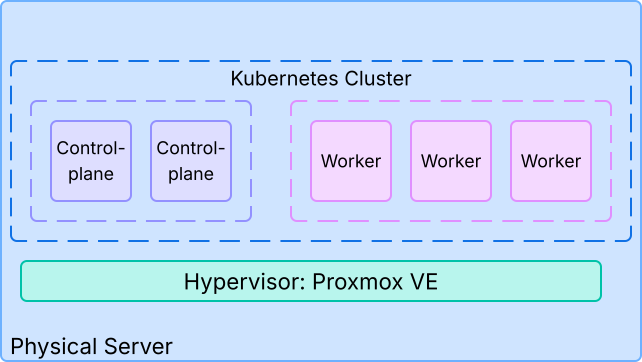
\includegraphics[width=0.7\textwidth]{k8s-cluster}
	\caption{Kubernetes cluster με δύο \textit{controlplane} κόμβους και τρεις
	\textit{κόμβους}} \label{fig:k8s-cluster}
\end{figure}

\subsection{Αυτοματισμοί υποδομής και διακυβέρνηση}

Όλα τα στοιχεία της πλατφόρμας ορίζονται δηλωτικά, με \textit{Helm charts} και
manifests που αποθηκεύονται σε κεντρικό αποθετήριο. Οι αλλαγές εφαρμόζονται
μέσω τυπικών ροών \textit{GitOps}: κάθε commit που επιφέρει αλλαγές στην υποδομή
<<ειδοποιεί>> έμμεσα έναν \textit{controller}, ο οποίος παρακολουθεί το
repository και συγχρονίζει την επιθυμητή κατάσταση με την τρέχουσα κατάσταση
του \textit{cluster}. Η πρακτική αυτή εξασφαλίζει ότι το \textit{production cluster}
αποτελεί ακριβές στιγμιότυπο του δηλωτικού μοντέλου, διευκολύνοντας την
auditability και την αναπαραγωγή σφαλμάτων.

Σε επίπεδο ασφάλειας, η πλατφόρμα οργανώνεται σε διακριτά \textit{Namespaces}
με αντίστοιχους κανόνες \textit{RBAC}, ώστε κάθε συνιστώσα να λειτουργεί εντός
περιορισμένου επιχειρησιακού πλαισίου. Η λογική αυτή ακολουθεί την καθιερωμένη
αρχή του «ελάχιστου απαιτούμενου δικαιώματος» και επιτρέπει στις υπηρεσίες να
εκτελούν μόνο τις λειτουργίες που τους αναλογούν, χωρίς να αποκτούν πρόσβαση σε
μη σχετιζόμενα υποσυστήματα. Η απομόνωση αυτή αποτελεί ικανοποιητικό επίπεδο
προστασίας για το scope της παρούσας εργασίας και διατηρεί τις υπηρεσίες πλήρως
ανεξάρτητες σε ό,τι αφορά την ανάπτυξη, τη συντήρηση και την παρακολούθησή
τους.

\section{Ροή δεδομένων σε πραγματικό χρόνο}

\subsection{Πηγές ροής δεδομένων}

Η αξιόπιστη και χαμηλής καθυστέρησης επεξεργασία ροών δεδομένων σε περιβάλλοντα
γεωργίας ακρίβειας προϋποθέτει τη διαχείριση ετερογενών πηγών, από θερμόμετρα
εδάφους έως αισθητήρες υγρασίας και \textit{pH}. Κάθε συσκευή εκτελεί το δικό
της ελαφρύ πρόγραμμα τηλεμετρίας, το οποίο υποστηρίζει διαφορετικές συχνότητες
εκπομπής και μπορεί να ρυθμιστεί ανάλογα με τη λειτουργική ανάγκη του
παραγωγού. Η πλατφόρμα παρέχει στον αισθητήρα τα απαραίτητα διαπιστευτήρια και
τις παραμέτρους λειτουργίας του, συμπεριλαμβανομένης της επιθυμητής granularity
του μηνύματος (π.χ.\ ανά 5, 30 ή 120 δευτερόλεπτα), ώστε κάθε συσκευή να
αποστέλλει δεδομένα με τρόπο προσαρμοσμένο στο προφίλ καλλιέργειας και στο
διαθέσιμο δίκτυο. Τα μηνύματα αποστέλλονται σε μορφή JSON μέσω \textit{MQTT}
και φτάνουν στο ingestion layer της πλατφόρμας με τη μορφή που τα εκπέμπει η
συσκευή, χωρίς ενδιάμεση τροποποίηση. Από εκεί και πέρα η ροή δεδομένων
δρομολογείται προς τα κατάλληλα topics και pipelines για περαιτέρω επεξεργασία,
όπως περιγράφεται στις επόμενες υποενότητες.

\subsection{Τεχνολογίες Streaming}

Στην προηγούμενη ενότητα παρουσιάστηκε το \textit{Apache Kafka} ως το βασικό
μέσο ενδιάμεσης επικοινωνίας μεταξύ των στοιχείων της πλατφόρμας. Σενάρια
\textit{streaming}, όπως αυτό της πλατφόρμας \textit{Nostradamus}, βασίζονται
στο \textit{Kafka} ως τον κεντρικό κόμβο του συστήματος, ο οποίος λειτουργεί ως
η κύρια <<πηγή αλήθειας>> για όλα τα υποσυστήματα. Κάθε γεγονός που συμβαίνει
στο σύστημα καταγράφεται αρχικά στο \textit{Kafka}, και στη συνέχεια κάθε
μικροϋπηρεσία εγγράφεται στο αντίστοιχο <<θέμα>> (\textit{topic}) ώστε να
λαμβάνει μόνο τα μηνύματα που της είναι απαραίτητα. Με αυτόν τον τρόπο
επιτυγχάνεται ο σαφής διαχωρισμός ανάμεσα στη ροή δεδομένων σε πραγματικό χρόνο
και στην κατανάλωση των μηνυμάτων. Συνεπώς, η σωστή σχεδίαση της υποδομής
συλλογής και μεταφοράς δεδομένων έως το \textit{Kafka} είναι κρίσιμη, καθώς από
εκεί και πέρα ο διαμοιρασμός τους στα υπόλοιπα υποσυστήματα γίνεται με απλό και
αποδοτικό τρόπο.

Για το \textit{deployment} του \textit{Kafka} στην πλατφόρμα επιλέχθηκε το
μοτίβο του \textit{Kubernetes Operator}, με στόχο την υψηλή διαθεσιμότητα, την
ανθεκτικότητα σε αστοχίες και την αυτοματοποιημένη διαχείριση του κύκλου ζωής
του συστήματος. Συγκεκριμένα, χρησιμοποιήθηκε ο \textit{Strimzi Kafka
Operator}, ο οποίος παρέχει πλήρη αυτοματοποίηση στην εγκατάσταση, ρύθμιση,
κλιμάκωση και αναβάθμιση των brokers, καθώς και στη διαχείριση των
\textit{topics} και των \textit{users}. Με αυτόν τον τρόπο αξιοποιούνται τα
πλεονεκτήματα του Kubernetes, όπως η ευκολία κλιμάκωσης, η αυτόματη
αποκατάσταση υπηρεσιών και η συνεπής διαχείριση πόρων, εξασφαλίζοντας παράλληλα
σταθερή και αποδοτική λειτουργία της υποδομής ροών. Τέλος, ο \textit{operator}
αυτός επιτρέπει την διαχείριση της υποδομής του \textit{Kafka} μέσω
\textit{GitOps} πρακτικών, γεγονός που ευθυγραμμίζεται με τις υπόλοιπες αρχές
και πρότυπα σχεδίασης της παρούσας εργασίας.

Είναι πλέον καθιερωμένη πρακτική οι αισθητήρες και γενικότερα οι χαμηλής
κατανάλωσης μικροελεγκτές που χρησιμοποιούνται σε υποδομές \textit{IoT} να
αποστέλλουν τα μηνύματά τους μέσω του πρωτοκόλλου \textit{MQTT}, καθώς αυτό
εξοικονομεί ενέργεια και επιτρέπει αποδοτική μετάδοση δεδομένων. Για την
εισαγωγή των μηνυμάτων αυτής της μορφής στο \textit{Kafka} απαιτείται η ύπαρξη
μηχανισμού γεφύρωσης. Στο πλαίσιο αυτό, αξιοποιήθηκε αρχικά το \textit{Strimzi
MQTT bridge}.

Ωστόσο, η ενσωματωμένη υλοποίηση του \textit{Strimzi} δεν υποστηρίζει ασφαλή
μεταφορά μέσω \textit{MQTTs}, γεγονός που αποτελεί κρίσιμο ζήτημα για την
παρούσα πλατφόρμα, δεδομένου ότι οι αισθητήρες βρίσκονται σε εξωτερικά δίκτυα.
Για την επίλυση του προβλήματος, ενσωματώθηκε ένας \textit{EMQX broker}, ο
οποίος λειτουργεί ως ασφαλής πύλη (\textit{secure gateway}) μεταξύ των
εξωτερικών συσκευών και του \textit{Kafka}, παρέχοντας υποστήριξη για
κρυπτογράφηση και μηχανισμούς πιστοποίησης σύμφωνα με τις απαιτήσεις της
αρχιτεκτονικής. Παράλληλα, ο \textit{EMQX broker} παρέχει δυνατότητες
φιλτραρίσματος βάσει των εισερχόμενων \textit{MQTT topics} και αντιστοίχισης
(\textit{mapping}) αυτών σε \textit{Kafka topics}, ώστε να προωθούνται στο
\textit{Kafka} μόνο τα απαραίτητα μηνύματα και να διατηρείται συνεπής η
ονοματολογία και η δομή των θεμάτων στην πλατφόρμα.

Η επιλογή του Kafka ως κεντρικού μηχανισμού μεταφοράς δεδομένων δικαιολογείται
και από τη φύση των γεωργικών συστημάτων, όπου παρατηρείται συχνά συνδυασμός
διαλείπουσας συνδεσιμότητας, απότομων αλλαγών στον ρυθμό παραγωγής δεδομένων
και ανομοιογενών payloads. Η εγγυημένη σειρά παράδοσης και η ανθεκτικότητα του
commit log καθιστούν το Kafka τον πλέον κατάλληλο μηχανισμό για ροές που
απαιτούν επαναληψιμότητα και ανοχή σε αστοχίες, ανεξαρτήτως του backend που
καταναλώνει τα μηνύματα.

\section{Προσωρινή αποθήκευση και cache drivers}

\subsection{Αρχιτεκτονική και ενσωμάτωση}

Το επίπεδο προσωρινής αποθήκευσης υιοθετεί το πρότυπο \textit{cache-aside}, με
αυστηρά όρια χρόνου ζωής (TTL 120 δευτερολέπτων) και υλοποίηση ως διακριτή
διασύνδεση. Η επιλογή αυτή επιτρέπει την εναλλαγή υποστρωμάτων χωρίς αλλαγές
στον κώδικα της εφαρμογής, ενώ το ίδιο interface παρέχει ενιαία συλλογή
μετρικών και ιχνηλασιμότητα. Εκτός του \textit{Valkey}, έχουν δημιουργηθεί
adapters για \textit{Memcached} και \textit{Dragonfly}, τους οποίους η
πλατφόρμα ενεργοποιεί ακόμη και κατά τη διάρκεια πειραμάτων συγκριτικής
αξιολόγησης ή ως μηχανισμό εφεδρείας. Η ύπαρξη πολλαπλών drivers προσφέρει
επιχειρησιακή ευελιξία: σε περίπτωση που ένα υπόστρωμα προσωρινής αποθήκευσης
παρουσιάσει αυξημένη καθυστέρηση ή μειωμένη διαθεσιμότητα, ο controller
επιτρέπει την άμεση μετάβαση σε εναλλακτικό driver. Σε συνδυασμό με τις
\textit{readiness probes}, εξασφαλίζεται ότι οι διεπαφές των χρηστών όπως το
\textit{UI} και τα τρίτα συστήματα δεν βλέπουν ποτέ ασταθή κατάσταση.

\subsection{Επιλογή και συγκριτική αξιολόγηση υποστρωμάτων}

Η επιλογή των τριών επιμέρους υποστρωμάτων καθορίστηκε από κριτήρια
συμβατότητας, λειτουργικότητας και αναμενόμενης επίδοσης. Το \textit{Valkey}
υιοθετήθηκε ως αναφορά, καθώς αποτελεί την πλέον συμβατή και κοινοτικά
υποστηριζόμενη μετεξέλιξη του οικοσυστήματος Redis, με πλούσιο σύνολο δομών
δεδομένων και δυνατότητα scripting, στοιχεία απαραίτητα για μελλοντικές
λειτουργίες της πλατφόρμας. Το \textit{Dragonfly} επιλέχθηκε λόγω της
αρχιτεκτονικής του που εστιάζει στην ενιαία πολυνηματική αξιοποίηση της μνήμης
και στο περιορισμένο αποτύπωμα πόρων, ενώ διατηρεί συμβατότητα σε επίπεδο
πρωτοκόλλου με το Valkey/Redis, καθιστώντας την εναλλαγή πρακτικά διαφανή.
Τέλος, το \textit{Memcached} ενσωματώθηκε ως ελαφριά, εδραιωμένη λύση με
περιορισμένο σύνολο λειτουργιών, η οποία όμως προσφέρει προβλέψιμη καθυστέρηση,
καθιστώντας την ιδανικό σημείο αναφοράς για συγκρίσεις καθαρού ρυθμού
διεκπεραίωσης.

Σημαντική παράμετρος της μελέτης είναι ότι το \textit{Valkey} και το
\textit{Dragonfly} μοιράζονται κοινό πρωτόκολλο και μοντέλο δεδομένων, γεγονός
που επιτρέπει την αξιολόγησή τους ως εναλλακτικές υλοποιήσεις της ίδιας λογικής
διασύνδεσης. Και τα δύο υποστρώματα παρέχουν μονόκλωνη σημασιολογία εκτέλεσης
εντολών, υποστηρίζουν scripting και σύνθετες δομές (δομές κατακερματισμού,
ταξινομημένα σύνολα), καθώς και χαρακτηριστικά όπως replication και μονιμότητα
δεδομένων. Κατά συνέπεια, τυχόν διαφοροποιήσεις στην επίδοση μπορούν να
αποδοθούν αποκλειστικά στην εσωτερική μηχανική υλοποίηση (μηχανή
κατακερματισμού, χρονοδρομολογητής, στρατηγικές χρήσης μνήμης) και όχι σε
αλλαγές του προγραμματιστικού μοντέλου. Η επιλογή τους επιτρέπει, επομένως, τη
συγκριτική απομόνωση των πλεονεκτημάτων που φέρει μια πιο επιθετική
πολυνηματική προσέγγιση (\textit{Dragonfly}) έναντι της κλασικής, πλήρως
συμβατής ερμηνείας (\textit{Valkey}), χωρίς να απαιτείται προσαρμογή του
εφαρμοστικού κώδικα.

\subsection{Πειραματικές υποθέσεις}

Πριν από την πειραματική διαδικασία διατυπώθηκαν συγκεκριμένα υποθετικά
σενάρια: αναμενόταν ότι το \textit{Memcached}, χάρη στο απλούστερο δυαδικό
πρωτόκολλο και την απουσία σύνθετων δομών, θα υπερτερεί σε P95 καθυστέρηση
ανάγνωσης και εγγραφής όταν το φορτίο είναι πλήρως συμμετρικό. Αντίστοιχα, η
υπόθεση για το \textit{Valkey} ήταν ότι θα εμφανίσει υψηλότερη σταθερότητα υπό
παρατεταμένα φορτία και καλύτερη συμπεριφορά σε σενάρια με ανάγκη αδιαίρετων
λειτουργιών. Για το \textit{Dragonfly}, η αναμενόμενη συμπεριφορά τοποθετήθηκε
ενδιάμεσα: στόχος ήταν να επαληθευθεί αν ο πολυνηματικός χρονοδρομολογητής και
η διαχείριση μνήμης που διαθέτει οδηγούν σε ρυθμό διεκπεραίωσης συγκρίσιμο με
το \textit{Memcached}, διατηρώντας παράλληλα τη λειτουργική πληρότητα του
\textit{Valkey}. Οι υποθέσεις αυτές καταγράφονται εδώ προκειμένου να
συσχετιστούν στη συνέχεια με τα αποτελέσματα του
Κεφαλαίου~\ref{chap:experiments}.

Η διατύπωση των παραπάνω υποθέσεων δεν στοχεύει απλώς στη σύγκριση διαφορετικών
υλοποιήσεων, αλλά και στην αξιολόγηση του κατά πόσο η πλατφόρμα μπορεί να
υποστηρίξει ετερογενείς drivers χωρίς αλλαγές στην επιχειρησιακή λογική. Η
προσέγγιση αυτή επιτρέπει τον διαχωρισμό της λειτουργικότητας της εφαρμογής από
τις επιδόσεις του υποστρώματος, στοιχείο που αποτελεί κρίσιμο παράγοντα για την
επεκτασιμότητα της πλατφόρμας σε μελλοντικά περιβάλλοντα και διαφορετικά
workloads.

\subsection{Στρατηγικές caching}

Η υιοθέτηση μηχανισμών κρυφής μνήμης σε κατανεμημένα συστήματα συνοδεύεται από
διαφορετικά πρότυπα (\textit{patterns}) υλοποίησης, καθένα από τα οποία φέρει
πλεονεκτήματα και περιορισμούς. Τα συνηθέστερα είναι τα ακόλουθα:

\subsubsection{Read-through}

Στο πρότυπο αυτό, όλες οι αναγνώσεις δεδομένων γίνονται μέσω της cache. Σε
περίπτωση που το ζητούμενο κλειδί δεν υπάρχει, η ίδια η cache αναλαμβάνει να
ανακτήσει τα δεδομένα από τη βάση και να τα αποθηκεύσει πριν τα επιστρέψει στον
χρήστη. Το πλεονέκτημα είναι η απλοποίηση της εφαρμογής, καθώς η λογική
ανάκτησης μετατίθεται στο cache layer. Ωστόσο, απαιτείται στενή ενσωμάτωση της
cache με τη βάση, κάτι που δυσχεραίνει την παραμετροποίηση σε περιβάλλοντα με
ετερογενείς πηγές δεδομένων.

\subsubsection{Write-through}

Σε αυτήν τη στρατηγική, κάθε εγγραφή περνάει πρώτα από την cache και στη
συνέχεια στη βάση δεδομένων. Η μέθοδος αυτή εξασφαλίζει συνεπή δεδομένα, καθώς
cache και βάση ενημερώνονται ταυτόχρονα, αλλά αυξάνει τον χρόνο απόκρισης για
κάθε write. Επιπλέον, το συνολικό throughput περιορίζεται από τον πιο αδύναμο
(αργό) κρίκο της αλυσίδας.

\subsubsection{Write-behind (ή Write-back)}

Τα δεδομένα γράφονται αρχικά μόνο στην cache και σε δεύτερο χρόνο, με ασύγχρονο
τρόπο, προωθούνται στη βάση. Το σχήμα αυτό προσφέρει υψηλές επιδόσεις για
σενάρια έντονου write load, αλλά εισάγει κινδύνους απώλειας δεδομένων σε
περίπτωση αστοχίας της cache, ενώ η βάση ενδέχεται να μην αντικατοπτρίζει την
πιο πρόσφατη κατάσταση.

\subsubsection{Cache-aside (ή Lazy loading)}

Στο πρότυπο αυτό, η εφαρμογή ελέγχει πρώτα την cache. Αν τα δεδομένα υπάρχουν,
επιστρέφονται άμεσα. Αν όχι, η εφαρμογή ανατρέχει στη βάση δεδομένων,
επιστρέφει τα αποτελέσματα στον χρήστη και ταυτόχρονα τα εισάγει εκ νέου στην
cache για μελλοντική χρήση. Το κύριο πλεονέκτημα είναι η απλότητα: η cache
λειτουργεί ως προαιρετικό επιταχυντικό στρώμα, χωρίς να απαιτείται βαθιά
ενσωμάτωση με τη βάση δεδομένων. Το μειονέκτημα είναι ότι τα δεδομένα μπορεί να
είναι στιγμιαία \textit{stale}, ειδικά σε περιπτώσεις έντονων ενημερώσεων.

\medskip Για τις ανάγκες της παρούσας πλατφόρμας, επιλέχθηκε το πρότυπο
\textit{cache-aside}, καθώς τα ερωτήματα αφορούν κυρίως αναγνώσεις πρόσφατων
τιμών αισθητήρων με χαμηλή πιθανότητα συνεχών τροποποιήσεων. Με τον τρόπο αυτό,
η ScyllaDB παραμένει η πηγή αλήθειας (\textit{source of truth}), ενώ το Valkey
cluster χρησιμοποιείται για να μειώσει τον χρόνο απόκρισης σε συχνά αιτήματα,
επιτυγχάνοντας ισορροπία ανάμεσα σε απόδοση και συνέπεια.

\section{Επίπεδο υπηρεσιών και εφαρμογής}

Το επίπεδο υπηρεσιών συγκροτείται γύρω από ένα κεντρικό API gateway, το οποίο
αποτελεί τη βασική διεπαφή των χρηστών και των downstream συστημάτων με τα
στοιχεία της πλατφόρμας. Η σχεδίασή του ακολουθεί modular αρχιτεκτονική, με
σαφή διαχωρισμό ευθυνών ανάμεσα στη διαχείριση πόρων, την επεξεργασία ροών, την
προσωρινή αποθήκευση και την παρατηρησιμότητα.

\subsection{Valkey cluster}

Η υποστήριξη του μηχανισμού cache υλοποιείται με \textit{Valkey cluster}, ο
οποίος αναπτύχθηκε μέσω του \textit{Hyperspike Operator}. Η λύση αυτή
εξασφαλίζει οριζόντια κλιμάκωση και υψηλή διαθεσιμότητα σε περιβάλλον
Kubernetes, με αυτοματοποιημένη διαχείριση των κόμβων Redis/Valkey.

Συνδυάζοντας τον Valkey cluster για ταχύτατη εξυπηρέτηση πρόσφατων μετρήσεων με
τη ScyllaDB για ανθεκτική και αναλυτική αποθήκευση, η πλατφόρμα διατηρεί
ισορροπία ανάμεσα σε χαμηλή καθυστέρηση και αξιοπιστία δεδομένων.

\begin{figure}[H]
	\centering
	\includegraphics[width=0.7\textwidth]{cache-aside}
	\caption{Λογικό διάγραμμα του προτύπου \textit{cache-aside}:
		το API ελέγχει αρχικά την κρυφή μνήμη (Valkey) για την αναζήτηση
		δεδομένων και, σε περίπτωση αποτυχίας, προσφεύγει στη ScyllaDB.
		Τα δεδομένα επιστρέφονται στον χρήστη και ταυτόχρονα επανεισάγονται
		στην cache, ώστε να εξυπηρετηθούν με χαμηλή καθυστέρηση σε επόμενα
		αιτήματα.}
	\label{fig:cache-aside-diagram}
\end{figure}

\subsection{API gateway και διαχείριση πόρων}

Το API παρέχει REST endpoints για την εγγραφή αγροτεμαχίων, την ενεργοποίηση
αισθητήρων, την έκδοση διαπιστευτηρίων και την προβολή συγκεντρωτικών τιμών
μέσω του \texttt{/aggregate}. Το API ελέγχει τα δικαιώματα κάθε κλήσης,
χαρτογραφεί τα αιτήματα σε συγκεκριμένα pipelines και επιβάλλει πολιτικές που
προκύπτουν από την ανάλυση των επιχειρησιακών ροών.

Η αρχιτεκτονική του API στηρίζεται σε διακριτά πακέτα: ένα για την πρόσβαση στη
βάση \textit{Scylla}, ένα για το caching layer, ένα για τη δρομολόγηση
αιτημάτων, καθώς και βοηθητικές βιβλιοθήκες για serialization, logging και
ιχνηλασιμότητα. Η επικοινωνία με τη Scylla υλοποιείται μέσω του οδηγού
\texttt{gocql}, ενώ το caching layer υλοποιείται ως ανεξάρτητο module
αποσυνδεδεμένο από τον αποθηκευτικό μηχανισμό.

\subsection{Διαχείριση Arroyo pipelines}

Η πλατφόρμα \textit{Arroyo} χρησιμοποιείται ως βασικό στοιχείο του streaming
layer, καθώς παρέχει connectors από \textit{Kafka} προς \textit{Scylla} σε
λειτουργία συνεχούς επεξεργασίας. Το API οργανώνει τα \textit{pipelines}
χρησιμοποιώντας abstractions που αντιστοιχούν σε αγροτεμάχια και αισθητήρες.
Μόλις καταχωρηθεί μία νέα συσκευή ή καταφτάσουν δεδομένα, ο controller
δημιουργεί δυναμικά το αντίστοιχο Arroyo job, το συνδέει με το κατάλληλο
\textit{topic} και παρακολουθεί το throughput του. Αν ένα job τερματιστεί, η
υπηρεσία αναλαμβάνει την αυτόματη επανεκκίνησή του και την ενημέρωση των
καταναλωτών, εξασφαλίζοντας \textit{self-healing} συμπεριφορά πέρα από τα όρια
του Kubernetes.

Παρότι σήμερα το Arroyo αξιοποιείται κυρίως ως connector, η σχεδίαση του API
επιτρέπει τη μελλοντική έκθεση επιπλέον λειτουργιών σε προχωρημένους χρήστες ή
σε DSL που θα πατήσει στο ίδιο API. Με αυτόν τον τρόπο ο κεντρικός έλεγχος
παραμένει στους developers της πλατφόρμας, αλλά παρέχεται σαφές σημείο
επέκτασης για πιο πολύπλοκα υπολογιστικά pipelines.

\subsection{Ανθεκτικότητα και ανοχή σε σφάλματα}

Στο API λειτουργούν controllers (υλοποιημένοι ως goroutines), οι οποίοι:

\begin{itemize}
	\item παρακολουθούν τις καταστάσεις των Arroyo jobs,
	\item αναδημιουργούν pipelines όταν απαιτείται,
    	\item συγχρονίζουν connectors μεταξύ Kafka και Scylla,
    	\item διασφαλίζουν ότι καμία ροή δεν μένει ανεπεξέργαστη.
\end{itemize}

Με αυτόν τον τρόπο η υπηρεσία επιτυγχάνει self-healing συμπεριφορά, η οποία
υπερβαίνει την αυτόματη αποκατάσταση που προσφέρει το Kubernetes.

\subsection{Υπηρεσία \textit{/aggregate} και caching layer}

Η προβολή συγκεντρωτικών μετρήσεων αποτελεί αναπόσπαστο κομμάτι κάθε συστήματος
που επεξεργάζεται δεδομένα αισθητήρων σε πραγματικό χρόνο. Παρότι η πλατφόρμα
διατηρεί αναλυτική ροή μέσω των pipelines, οι περισσότεροι παραγωγοί και
εφαρμογές καταναλώνουν τα δεδομένα σε συνοπτική μορφή, σε παράθυρα
συγκεκριμένης διάρκειας και για συγκεκριμένο τύπο αισθητήρα. Για τον λόγο αυτόν
σχεδιάστηκε η υπηρεσία \textit{/aggregate}, η οποία λειτουργεί ως ενιαίο σημείο
πρόσβασης για την εξαγωγή απλοποιημένων στατιστικών (π.χ.\ ελάχιστο, μέγιστο,
μέσο όρο) πάνω σε πρόσφατα δεδομένα. Η υπηρεσία αυτή αναλαμβάνει να
εξυπηρετήσει τα πιο συχνά αναγνώσιμα workloads της πλατφόρμας με προβλέψιμο
latency, αξιοποιώντας το caching layer και τις μετρικές παρατηρησιμότητας που
έχουν ενσωματωθεί. Κάθε κλήση δέχεται παραμέτρους παραθύρου (π.χ. 1 ώρα) και
τύπο αισθητήρα (θερμοκρασία, υγρασία, \textit{pH}), επιστρέφοντας ταυτόχρονα
\textit{min}, \textit{max} και \textit{average} τιμές. Η υλοποίηση ακολουθεί
μοτίβο \textit{cache-aside}: αρχικά επιχειρείται \textit{CacheFetch}, στη
συνέχεια γίνεται \textit{DBFetch} από τη \textit{Scylla} μόνο αν υπάρξει
\textit{miss}, και τέλος τα αποτελέσματα αποθηκεύονται με TTL 120
δευτερολέπτων. Ο κύκλος αυτός είναι πλήρως ορατός μέσω traces, ενώ οι σχετικές
μετρικές τροφοδοτούν τα dashboards που χρησιμοποιήθηκαν και στα πειράματα.

Το caching layer είναι ανεξάρτητη βιβλιοθήκη με κοινό interface, στην οποία
έχουν αναπτυχθεί drivers για \textit{Valkey}, \textit{Memcached} και
\textit{Dragonfly}. Ο εκάστοτε driver επιλέγεται με παραμετροποίηση στο
\textit{deployment}, γεγονός που επέτρεψε τη γρήγορη εκτέλεση των benchmark
σεναρίων και την ανάλυση των P95 καθυστερήσεων. Παράλληλα, ο ίδιος μηχανισμός
καταγράφει \textit{cache hit/miss} με granularity ανά αισθητήρα και είδος
aggregation, επιτρέποντας την αξιολόγηση της αποδοτικότητας του caching ανά
workload. Ως μελλοντική βελτίωση σχεδιάζεται ένα ταχύτερο endpoint μεταφοράς
δεδομένων μεταξύ υπηρεσιών, ώστε να παρακάμπτει πλήρως το UI όταν απαιτείται
ενδοσυστημική ολοκλήρωση.

Η συγκεκριμένη υπηρεσία λειτουργεί, επιπλέον, ως αντιπροσωπευτικό υπόδειγμα του
συνολικού τρόπου με τον οποίο η πλατφόρμα χειρίζεται δεδομένα αισθητήρων. Το
\textit{/aggregate} προσφέρει ένα πλήρως λειτουργικό σημείο δοκιμής για το
caching layer, καθιστώντας εφικτή την αξιολόγηση διαφορετικών drivers και τη
μέτρηση της συμπεριφοράς τους κάτω από πραγματικό φόρτο. Ως εκ τούτου, η
υπηρεσία διαδραματίζει διττό ρόλο: από τη μία επιτρέπει την άμεση κατανάλωση
συγκεντρωτικών μετρήσεων από τους παραγωγούς, και από την άλλη παρέχει ένα
σταθερό και επαναλήψιμο περιβάλλον για benchmarking, debugging και ανάλυση των
επιδόσεων της υποδομής. Παρότι το \textit{/aggregate} καλύπτει τις βασικές
ανάγκες του τρέχοντος συστήματος, η υφιστάμενη αρχιτεκτονική επιτρέπει τη
δημιουργία επιπλέον endpoints με παρόμοια λογική, είτε για πιο σύνθετες
αναλύσεις είτε για επέκταση σε νέα είδη αισθητήρων και νέους τύπους χρονικών
ερωτημάτων, μετατρέποντας σταδιακά την πλατφόρμα σε πλήρες εργαλείο προβολής
και επεξεργασίας γεωργικών δεδομένων σε πραγματικό χρόνο.

\subsection{Frontend και διεπαφές παρακολούθησης}

Παρότι το κύριο βάρος της εργασίας εστιάζει στα υποσυστήματα υποδομής,
επεξεργασίας ροών και προσωρινής αποθήκευσης, η ύπαρξη ενός λειτουργικού
frontend κρίθηκε απαραίτητη ώστε να αναδεικνύονται στην πράξη οι δυνατότητες
του API και του caching layer. Το frontend λειτουργεί ως το πρώτο σημείο επαφής
των παραγωγών με την πλατφόρμα και αποτελεί ένα ελαφρύ, πλήρως λειτουργικό
παράδειγμα κατανάλωσης των υπηρεσιών που περιγράφηκαν στις προηγούμενες
ενότητες. Πρακτικά, χρησιμεύει ως «βιτρίνα» της αρχιτεκτονικής: επιτρέπει την
ορατή επαλήθευση της ροής δεδομένων, της συμπεριφοράς του \textit{/aggregate}
και της απόδοσης του caching layer, χωρίς να απαιτούνται ειδικά εργαλεία ή
σύνθετα dashboard setups.

Το UI καταναλώνει το API gateway και παρέχει φόρμες για την εγγραφή
αγροτεμαχίων, την ενεργοποίηση αισθητήρων και την διαχείριση των ρυθμίσεών
τους. Εμφανίζει επίσης τις πιο πρόσφατες μετρήσεις ανά σημείο, αξιοποιώντας
άμεσα τα αποτελέσματα της υπηρεσίας \textit{/aggregate}. Με αυτόν τον τρόπο το
frontend λειτουργεί και ως δείκτης ορθής λειτουργίας του caching layer, αφού η
διαφορά μεταξύ cache hits και misses αποτυπώνεται άμεσα στον χρόνο απόκρισης
του UI.

Πέρα από τις βασικές ροές onboarding, το frontend παρέχει συνοπτικές μετρικές
που συνοψίζουν την τρέχουσα κατάσταση του αγρού, επιτρέποντας στον χρήστη να
λάβει μια γρήγορη εικόνα της δραστηριότητας των αισθητήρων. Για πιο αναλυτικά
KPIs, χρονοσειρές και διαγνωστικά στοιχεία, οι χρήστες ανακατευθύνονται στα
εξειδικευμένα Grafana boards, όπου συγκεντρώνονται οι μετρικές από το
monitoring stack της πλατφόρμας.

Ο σχεδιασμός του frontend κρατήθηκε εσκεμμένα απλός. Στόχος του δεν είναι να
αναπαράγει την πληρότητα ενός παραγωγικού dashboard, αλλά να λειτουργήσει ως
reference implementation πάνω στο API, διευκολύνοντας την ανάπτυξη νέων
υπηρεσιών και αποτελώντας σημείο εκκίνησης για μελλοντικές επεκτάσεις. Η
υφιστάμενη δομή επιτρέπει την προσθήκη πρόσθετων σελίδων και endpoints, από
εμπλουτισμένα γραφήματα μέχρι real-time feeds, χωρίς να απαιτούνται αλλαγές στο
υπόβαθρο της πλατφόρμας.

\section{Παρατηρησιμότητα}

Η παρατηρησιμότητα αποτελεί θεμελιώδες χαρακτηριστικό της πλατφόρμας, καθώς
επιτρέπει την πλήρη κατανόηση της συμπεριφοράς του συστήματος και την
επαλήθευση ότι η ροή των αισθητήριων δεδομένων λειτουργεί όπως αναμένεται. Η
παρούσα ενότητα αναλύει τους τρεις βασικούς άξονες παρατηρησιμότητας που
υλοποιήθηκαν: \textit{μετρικές}, \textit{καταγραφές} και
\textit{ιχνηλασιμότητα}.

\subsection{Μετρικές και SLI παρακολούθησης}

Η προσέγγιση με \textbf{προτεραιότητα στην παρατηρησιμότητα} ακολουθείται σε
όλα τα στοιχεία του συστήματος, ώστε η ροή των αισθητήριων δεδομένων να είναι
πλήρως μετρήσιμη και επαληθεύσιμη. Τα βασικά \textit{SLI} που παρακολουθούνται
είναι η καθυστέρηση ανάγνωσης και εγγραφής στην cache, ο δείκτης \textit{cache
miss} και ο χρόνος ανάγνωσης της βάσης \textit{Scylla}. Τα μεγέθη αυτά
εκτίθενται από τις υπηρεσίες μέσω \textit{Prometheus exporters} και
προβάλλονται σε ενιαία \textit{Grafana dashboards}, επιτρέποντας άμεση σύγκριση
μεταξύ διαφορετικών cache drivers ή διαφορετικών pipelines.

Η συλλογή σημάτων δεν περιορίζεται σε επίπεδο υποδομής. Κάθε κριτικό σημείο της
υπηρεσίας \textit{/aggregate} φέρει στοχευμένα \textit{metrics}, όπως ο χρόνος
ολοκλήρωσης των λειτουργιών \textit{CacheFetch}, \textit{DBFetch} και
\textit{CacheStore}, καθώς και αντιστοιχίσεις με το παράθυρο (π.χ. 15 λεπτά, 1
ώρα) και το είδος αισθητήρα (θερμοκρασία, υγρασία, pH). Με αυτόν τον τρόπο η
παρατηρησιμότητα διασταυρώνεται με το \textit{business logic} της πλατφόρμας
και τα πειραματικά αποτελέσματα μπορούν να χαρτογραφηθούν άμεσα σε συγκεκριμένα
workloads.

Η δυνατότητα συσχέτισης σημάτων από πολλαπλά επίπεδα, όπως ο χρόνος ανάγνωσης
cache, η καθυστέρηση επεξεργασίας στους brokers και ο τελικός χρόνος απόκρισης
του API, προσδίδει στην πλατφόρμα χαρακτηριστικά cross-layer παρατηρησιμότητας.
Τα συνδυαστικά αυτά σήματα διευκολύνουν την αναγνώριση συστημικών προβλημάτων
που δεν είναι εμφανή όταν μετρώνται απομονωμένα, όπως συμφόρηση I/O ή μη
ομοιόμορφη κατανομή φορτίου σε πυρήνες.

\subsection{Καταγραφές και διασταύρωση συμβάντων}

Πέρα από τις μετρικές, εφαρμόζεται τυποποιημένο σύστημα καταγραφής
(\textit{structured logging}) με εμπλουτισμό μεταδεδομένων και
\textit{correlation IDs}. Όλα τα logs ρέουν προς \textit{Grafana Loki},
επιτρέποντας πολυδιάστατη αναζήτηση ανά αισθητήρα, pipeline ή χρήστη. Η
διάσταση της ιχνηλασιμότητας αναλύεται εκτενώς στην υποενότητα «Ιχνηλασιμότητα
και ανάλυση αιτημάτων», όπου περιγράφεται ο τρόπος με τον οποίο τα traces
συμπληρώνουν τα παραπάνω σήματα.

Το σύστημα καταγραφής λειτουργεί συμπληρωματικά προς τις μετρικές: σε
περιπτώσεις απόκλισης χρόνου απόκρισης, τα logs παρέχουν το πλαίσιο (context)
και τα συμβάντα που οδήγησαν στη συγκεκριμένη συμπεριφορά.

\subsection{Ιχνηλασιμότητα και ανάλυση αιτημάτων}

Η πλήρης ιχνηλασιμότητα (\textit{tracing}) αποτελεί τον τρίτο πυλώνα της
παρατηρησιμότητας και επιτρέπει την αποσύνθεση κάθε αιτήματος σε επιμέρους
λειτουργικές φάσεις. Για τον σκοπό αυτόν χρησιμοποιήθηκε η βιβλιοθήκη
\textit{OpenTelemetry}, με δρομολόγηση των traces στην υπηρεσία \textit{Tempo}
του Grafana μέσω ενός \textit{OTLP gRPC} εξαγωγέα.

Η αρχικοποίηση του tracer provider γίνεται κατά την εκκίνηση της υπηρεσίας: ο
εξαγωγέας συνδέεται στο endpoint του Tempo, ενεργοποιείται ο batch processor
για αποδοτική αποστολή παρτίδων και ορίζεται \textit{resource} με
χαρακτηριστικά όπως το όνομα υπηρεσίας (\textit{nostradamus-api}). Η διαδικασία
αρχικοποίησης μεριμνά επίσης για την ασφαλή αποδέσμευση του tracer provider
κατά τον τερματισμό, ώστε να μη χαθούν spans που βρίσκονται σε εκκρεμότητα.

Σε επίπεδο εφαρμογής, κάθε κλήση στο \textιt{/aggregate} ξεκινά span με το
context του αιτήματος, επιτρέποντας την αλυσίδωση με downstream κλήσεις. Η
υπηρεσία καταγράφει χαρακτηριστικά που περιγράφουν τα βασικά query parameters
(αισθητήρας, παράθυρο, τύπος μετρήσεων) και αποτυπώνει την τελική κατάσταση με
βάση τους κωδικούς επιστροφής του \textit{OpenTelemetry} (π.χ. \textit{OK},
\textit{Error}). Τα σημεία ελέγχου που χειρίζονται σφάλματα παραμετρικών
ελέγχων ή επικοινωνίας με τη βάση δεδομένων συνοδεύουν το span με σχετικές
εγγραφές (\textit{recorded errors}) και εμπλουτισμένα logs, έτσι ώστε τα traces
να απεικονίζουν πλήρως το μονοπάτι που ακολουθήθηκε.

\subsubsection{Ιχνηλασιμότητα στο caching layer}

Ιδιαίτερη έμφαση δίνεται στην ενοποίηση της ιχνηλασιμότητας με το caching
layer. Κάθε driver (π.χ. \textit{Memcached}, \textit{Valkey}) δημιουργεί
δευτερεύοντα spans για τις λειτουργίες \textit{FetchAggregate} και
\textit{StoreAggregate}, μεταφέροντας το context του αρχικού HTTP αιτήματος. Τα
spans φέρουν κοινά attributes, όπως το είδος του driver, το cache key και τη
χρονική διάρκεια ζωής της εγγραφής. Επιπλέον, η ροή αποτυπώνει με σαφήνεια τα
αποτελέσματα (\textit{hit}, \textit{miss}, \textit{corrupt}) και όλες τις
συνθήκες σφάλματος, καθώς καταγράφονται μαζί με το αντίστοιχό τους status.

Έτσι, το τελικό trace απεικονίζει ολόκληρο το μονοπάτι CacheFetch $\rightarrow$
DBFetch $\rightarrow$ CacheStore, συμπεριλαμβανομένων των χρονικών μεγεθών που
παρακολουθούνται παράλληλα και από τα metrics.

\subsubsection{Πλεονεκτήματα της ενιαίας ιχνηλασιμότητας}

Η παραπάνω προσέγγιση έχει δύο σημαντικά πλεονεκτήματα. Πρώτον, επιτρέπει την
ταχεία συσχέτιση των χρονικών αποκλίσεων που εμφανίζονται στα dashboards με
συγκεκριμένες κλήσεις και παραμέτρους, γεγονός κρίσιμο για την κατανόηση των
P95 καθυστερήσεων. Δεύτερον, παρέχει πλήρη ορατότητα στο σύστημα cache-aside,
προσφέροντας στοιχεία για τη συμπεριφορά κάθε driver χωρίς να απαιτείται
ξεχωριστή υλοποίηση debugging.

Σε ευρύτερο πλαίσιο, η ιχνηλασιμότητα αποτελεί βασικό μηχανισμό αποσφαλμάτωσης
σε κατανεμημένα περιβάλλοντα, όπου οι πιθανές αιτίες καθυστέρησης δεν
εντοπίζονται σε μία μόνο διεργασία αλλά προκύπτουν από την αλληλεπίδραση
πολλαπλών μικροϋπηρεσιών. Η δυνατότητα οπτικοποίησης των spans επιτρέπει την
κατανόηση του πραγματικού data path και καθιστά εφικτή την απομόνωση αιχμών
καθυστέρησης που συνήθως καλύπτονται από αθροιστικές μετρικές.

\section{Ένταξη πελάτη}

Η διαδικασία onboarding λαμβάνει χώρα αποκλειστικά μέσω του API gateway. Αρχικά
ο παραγωγός καταχωρεί τα στοιχεία του αγροτεμαχίου και των αισθητήρων, ενώ
έπειτα μπορεί να λάβει τα διαπιστευτήρια του κάθε αισθητήρα. Στη συνέχεια, το
API δημιουργεί τα αντίστοιχα topics στο \textit{Kafka}, συνδέει το αγροτεμάχιο
με το κατάλληλο Arroyo pipeline και ενεργοποιεί τη ροή δεδομένων. Τέλος, το
caching layer ενημερώνει τα indices ώστε τα πρόσφατα δεδομένα να είναι
διαθέσιμα αμέσως στο UI.

\begin{figure}[H] \centering
	\includegraphics[width=0.7\textwidth]{client-onboarding-process}
	\caption{Διάγραμα δραστηριότητας για τη διαδικασία ένταξης νέου πελάτη}
	\label{fig:client-onboarding-activity}
\end{figure}
